\documentclass{bredelebeamer}
\usepackage{subfig}

%%%%%%%%%%%%%%%%%%%%%%%%%%%%%%%%%%%%%%%%%%%%%%%%
\title[Kubernetes]{Kubernetes}
% Titre du diaporama

\subtitle{manage application, not machines}
% Sous-titre optionnel

\author{N. Salleron B. Affes}
% La commande \inst{...} Permet d'afficher l' affiliation de l'intervenant.
% Si il y a plusieurs intervenants: Marcel Dupont\inst{1}, Roger Durand\inst{2}
% Il suffit alors d'ajouter un autre institut sur le modéle ci-dessous.

\date{Lundi 12 Février 2018}
% Optionnel. La date, généralement celle du jour de la conférence

\subject{NMV}
% C'est utilisé dans les métadonnes du PDF

\logo{

\includegraphics[scale=0.03]{images/logo.jpg}
}

%%%%%%%%%%%%%%%%%%%%%%%%%%%%%%%%%%%%%%%%%%%%%%%%%%%%%%%%%%%%%%%%%%%%%
\begin{document}

\begin{frame}
  \titlepage
\end{frame}

\begin{frame}{Sommaire}
  \tableofcontents
  % possibilité d'ajouter l'option [pausesections]
\end{frame}

\section{Introduction}
\subsection{Introduction}

\begin{frame}{Historique}
\begin{block}{Une longue émergence}
\begin{itemize}
\item Borg
	\begin{itemize}
	\item Démarrage en 2004.
	\item Développé en interne.
	\item Manager de containers.
	\item Objectif : réduction des coups en partageant machines et applications.
	\item \textbf{Non open-source.}
	\end{itemize}	\pause
\item Omega	
	\begin{itemize}
	\item Fils de Borg.
	\item Amélioration de l'écosystème apporté par Borg.
	\item  \textbf{Non open-source.}
	\end{itemize}   \pause
\item Kubernetes
	\begin{itemize}
	\item Adaptable à plusieurs infrastructure cloud.
	\item  \textbf{Open-source.}
	\end{itemize}
\end{itemize}
\end{block}
\end{frame}

\begin{frame}{Introduction}
%Texte normal \alert{Texte Alert}  \exemple{Texte exemple} \emph{Texte emphase}
\begin{columns}
\begin{column}{0.5\textwidth}

Nom venant du Grec, crée par 3 ingénieurs de chez Google en 2014.
\begin{itemize}
\item \textit{Orchestrateur} - Gestionnaire de conteneur.
\item Exécute et manages des containers.
\item Propose une API permettant la gestion de plusieurs clouds (Google, Microsoft, Amazon, et pleins d'autres).
\item 100\% Open Source écrit en Go.
\end{itemize}
\vspace{10px}
Il permet de se focus sur les applications et non sur le déploiement.  \\
Google exécute 2 milliards de conteneurs par semaine avec ces systèmes.\\
Dernière version : 1.9.3 (sorti il y a 3 jours) \\ 

\vspace{10px}
\textit{"manage application, not machines" - Tim Hockin}

\end{column}
\begin{column}{0.5\textwidth}
\begin{figure}
\centering

\includegraphics[scale=0.15]{images/img1.png}
\caption{Logo de Kubernetes}
\end{figure}
\end{column}
\end{columns}
\end{frame}

\begin{frame}{Popularité}
Évolution des recherches entre \textcolor{Framableu}{Kubernetes}, \textcolor{Framarouge}{Mesos}, \textcolor{Framajaune}{Docker Swarm}
\begin{center}
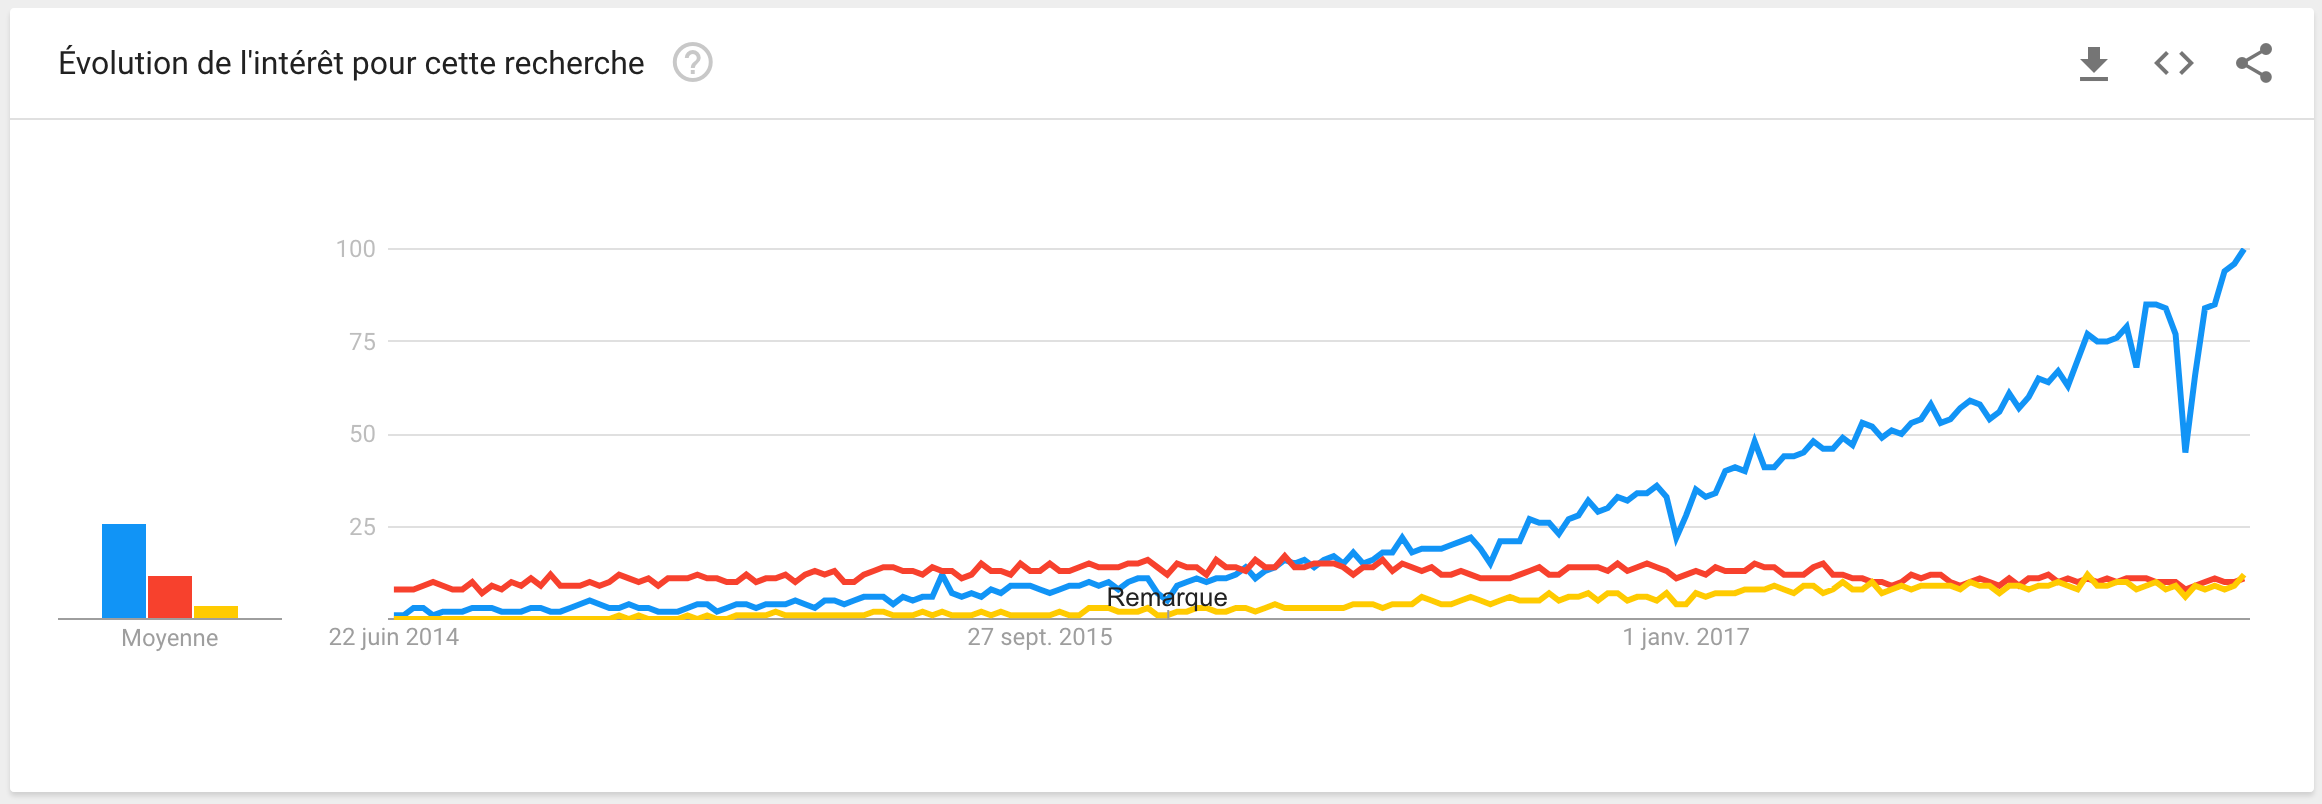
\includegraphics[scale=0.25]{images/img2.png}
\end{center}\pause
Une communauté très active : 
\begin{itemize}
\item Actuellement 61000 commits avec plus de 1500 contributeurs
\end{itemize}
\begin{center}
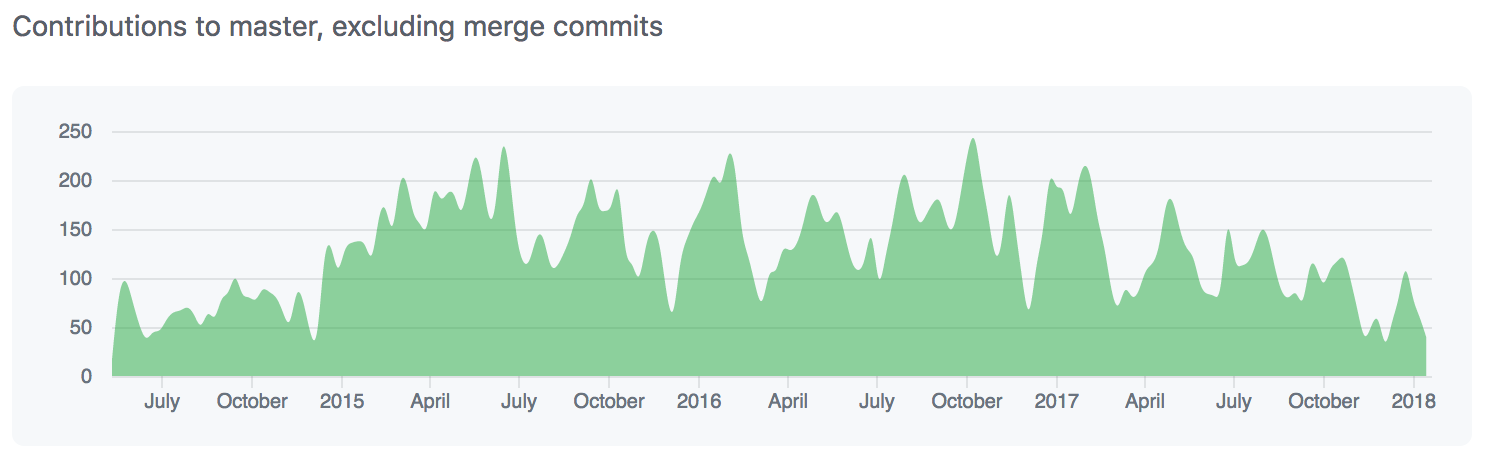
\includegraphics[scale=0.3]{images/img3.png}
\end{center}
\end{frame}

\section{Docker}
\subsection{Some few things about Docker}
\begin{frame}
\begin{center}

\includegraphics[scale=0.3]{images/img5.png}
\end{center}
\end{frame}
\begin{frame}
Docker est un conteneur léger, permettant de l'isolation entre les processus.
\begin{center}
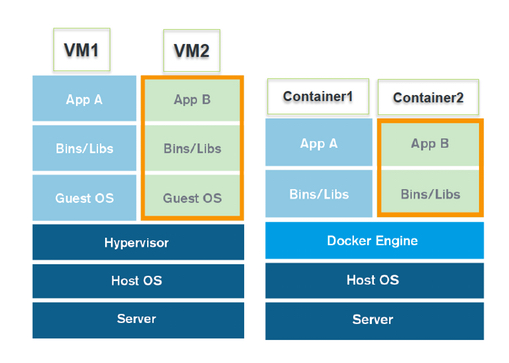
\includegraphics[scale=0.3]{images/img4.jpg}
\end{center}
\begin{itemize}
\item Retire le coût de la virtualisation (pas de gestion hardware)
\item Retire le coût d'exécution de plusieurs OS.
\end{itemize}

\end{frame}

\begin{frame}
Docker se base sur deux technologies du noyau : 
\begin{itemize}
\item CGroups
\item Namespace
\end{itemize} \pause

\begin{exampleblock}{Control Groups}
Feature kernel qui permet de contrôler, limité et isoler l'usage des ressources pour un processus ou une collection de processus. 
\end{exampleblock} \pause


\begin{block} {CGroups Isolation}
\begin{itemize}
\item  Quantitative Isolation : Les CGroups ne peuvent pas avoir plus de pages que la limite imposé.
\item Qualitative Isolation : Les CGroups doivent accéder à leur mémoire comme si elles étaient seules sur la machine.
\end{itemize}
\end{block} \pause

\begin{exampleblock}{Namespace}
Feature linux qui permet de créer une vue local pour les ressources d'un systèmes. Les ressources en dehors du namespace ne sont pas visible. 
\end{exampleblock}
\end{frame}


\section{Kubernetes  Core Concept}
\subsection{Core concept}

\begin{frame}{Kubernetes}
\begin{center}

\includegraphics[scale=0.3]{images/img6.png}
\end{center}
\end{frame}

\begin{frame}{Pods}

\begin{columns}
\begin{column}{0.5\textwidth}
\begin{figure}
\centering
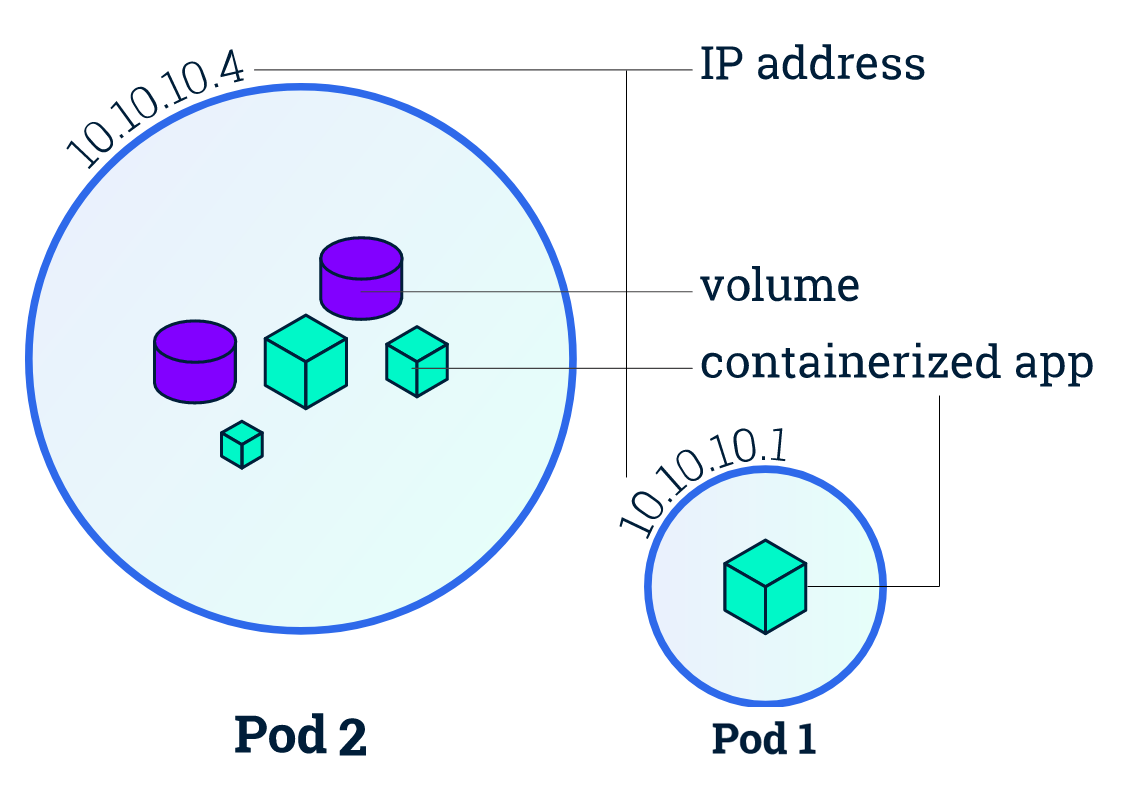
\includegraphics[scale=0.25]{images/img7.png}
\caption{Les Pod dans Kubernetes}
\end{figure}
\end{column}
\begin{column}{0.5\textwidth}
\begin{block}{Caractéristiques du Pod}

\begin{itemize}
\item Unité de base de l'ordonnancement. 											\pause
\item Vue abstraite de composants conteneurisés.								\pause
\item Il peut regrouper 1 ou * conteneurs. \\=> Couplage fort.				\pause
\item Chaque pod possède une adresse IP unique (limité au cluster).		\pause
\item Un Pod peut définir un volume. 
		%comme un répertoire sur un disque local ou réseau.
		Il a la même durée de vie que le Pod.
\end{itemize}
\end{block}																							\pause
\end{column}



\end{columns}
\vspace{4px}
Bénéfices du pod : 
\begin{itemize}
\item Plusieurs conteneurs dans 1 Pod\\
=> Processus qui ont besoin d'interroger un autre processus avec une faible latence.		\pause
\item Utilisable sous plusieurs environnements (configuration via JSONDoc)		\pause
\item Mortel : un container peut mourir.		\pause
\end{itemize}
\end{frame}



%Kubernetes permet à des clients (utilisateurs et composants internes) d'attacher des paires clés-valeurs appelées "labels" à n'importe quel objet d'API dans le système, par exemple les pods et les nodes. Par correspondance, les "label selectors" sont des interrogations faites sur les labels en lien avec des objets15.

%Labels et selectors constituent le premier mécanisme de groupement dans Kubernetes, et sont utilisés pour déterminer les composants sur lesquels appliquer une opération18.

%Par exemple, si les Pods d'une application ont des labels pour un système tier ("front-end", "back-end", par exemple) et une release_track ("preproduction", "production", par exemple), alors une opération sur tous les nodes "back-end" et "preproduction" peuvent utiliser un label selector comme suit19 :

%    tier=back-end AND release_track=preproduction

\begin{frame}{Label et Selector}



\end{frame}





\begin{frame}{Contrôleurs}






\end{frame}




\begin{frame}{Services}




\end{frame}

\section{Kubernetes Architecture Concept}
\subsection{Architecture concept}

\begin{frame}{Kubernetes Master}
\end{frame}

\begin{frame}{Kubernetes Node}
\end{frame}



\end{document}




